\documentclass[a4paper,12pt]{article}

\usepackage[utf8]{inputenc}

\usepackage[parfill]{parskip}

\usepackage[T1]{fontenc}
\usepackage[french]{babel}
\usepackage{array,multirow,makecell}
\usepackage{longtable}
\usepackage{setspace}
\usepackage{makecell}
\setcellgapes{1pt}
\makegapedcells
\usepackage[table]{xcolor}
\renewcommand*{\emph}[1]{\textcolor{green}{#1}}
\newcolumntype{R}[1]{>{\raggedleft\arraybackslash }b{#1}}
\newcolumntype{L}[1]{>{\raggedright\arraybackslash }b{#1}}
\newcolumntype{C}[1]{>{\centering\arraybackslash }b{#1}}
\usepackage{amsfonts}
\usepackage{fullpage}
\usepackage{graphicx}
\usepackage{float}
\usepackage{geometry}
\usepackage{amsmath}
\usepackage{amssymb}
\usepackage{xspace}
\usepackage{epstopdf}
\usepackage{tabularx}

% -----------------------------------------------------
\begin{document}

    \begin{titlepage}

        \begin{center}
        
            \begin{figure}[H]
              \begin{minipage}[c]{.46\linewidth}
                    \centering
                    
\includegraphics[scale = 0.3]{images/ulb.png}
                \end{minipage}
                \hfill%
                \begin{minipage}[c]{.46\linewidth}
                    \centering
                    
\includegraphics[scale=0.5]{images/ulb2.jpg}
                \end{minipage}
            \end{figure}
        
            {\\[2 cm] \Huge\\INFO-F209 - Projets d'informatique 2 \\ \\ Software Requirements Document \\ [1 cm]
            L-type\\[2 cm]}
            {Aïssa ABDOUL-AZIZ \\[0,2 cm] Kokou ADEGNON \\[0,2 cm] Jeremy BARBER \\[0,2 cm] Helin DEMIREL \\[0,2 cm] Camelia ELKENZE \\[0,2 cm] Alexandre KINSOEN \\[0,2 cm] Salim LATOUNDJI \\[0,2 cm] Mario MASSIMETTI \\[0,2 cm] Martin VANNESTE \\ [3 cm] Décembre 2020}

        \end{center}

    \end{titlepage}

\newpage

\tableofcontents

\newpage

% ----------------------------------------------------

\section{Introduction}

L’objectif de ce projet consiste en la réalisation d'un jeu d'action de style shoot 'em up en multijoueur. Dans ce jeu, un ou deux joueurs doivent parcourir plusieurs niveaux en détruisant les ennemis qui se présentent devant eux, tout en esquivant les tirs provoqués par ces derniers. Les vaisseaux dirigés par les joueurs peuvent récupérer des bonus d’armement lâchés par leurs nombreux adversaires, pour mieux les éliminer. L'objectif des joueurs étant de terminer tous les niveaux sans que leur compteur de vies ne se retrouve à 0. En effet, un joueur en possède un nombre déterminé. Si un projectile d'un joueur touche un ennemi, son score est augmenté. À la fin d'une partie, le score de chaque utilisateur est mis à jour si celui-ci est meilleur que son score actuel.

En dehors du jeu, un utilisateur a la capacité de gérer sa liste d'amis et de consulter le classement général des joueurs.

Le jeu ne sera exécutable que sous le système d'exploitation Linux.

\subsection{Historique}
\begin{tabularx}{15cm}{|c|c|X|}
	\hline
		Dates & Sujets & Noms \\
	\hline
		13/11/20 & UseCase Utilisateur & Camelia, Jeremy, Salim \\
	\hline
		22/11/20 & Annexe & Jeremy, Camelia \\
	\hline
		10/12/20 & Besoins utilisateur & Kokou, Camelia, Helin, Aissa\\
	\hline
		11/12/20 & Version finale diagramme de classe  & Jeremy, Martin, Salim, Alexandre\\
	\hline
		14/12/20 & Version final des diagrammes de sequence & Helin, Aissa, Martin, Kokou, Camelia, 
		Mario, Alexandre, Jeremy, Salim\\
	\hline
		15/12/20 & Introduction du SRD & Helin, Aissa, Mario\\
	\hline
		15/12/20 & Besoins système partie serveur & Alexandre, Jeremy, Martin, Camelia, Aissa, Helin\\
	\hline
		15/12/20 & Besoins système partie client & Kokou, Mario, Salim\\
	\hline
		16/12/20 & Description du diagramme de classe & Helin, Mario, Salim, Aissa,
		Alexandre, Jeremy, Martin\\
	\hline

\end{tabularx}

\section{Besoins utilisateur}

\subsection{Besoins fonctionnels}

% ajoute de l'image

\begin{figure}[h!]
\centering
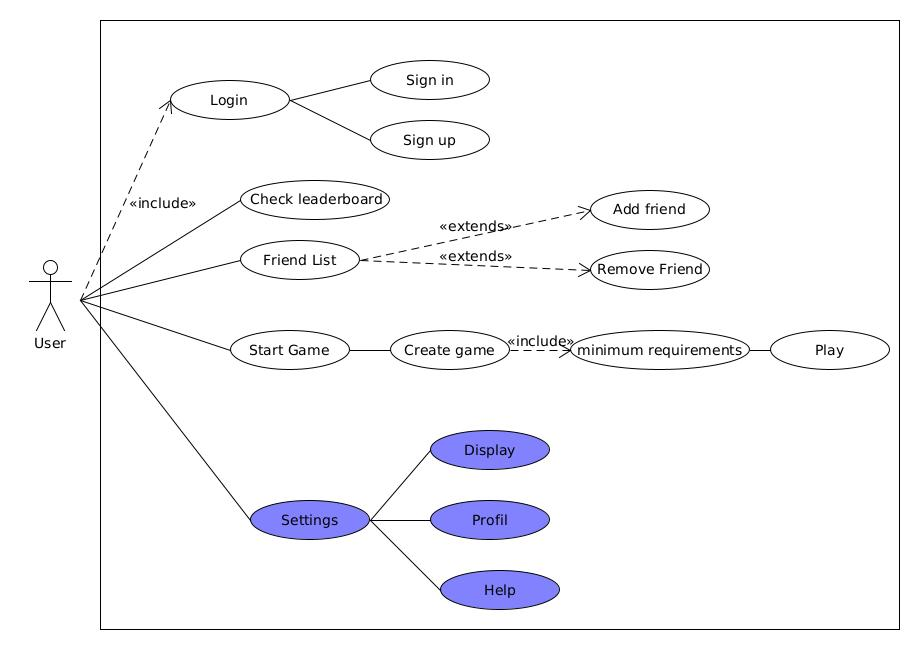
\includegraphics[width=15cm]{images/UserUseCase.jpg}
\caption{Diagramme de Use Case côté utilisateur}
\label{fig:UserUseCase}
\end{figure}

\subsubsection{Connexion}
En lançant le programme, l'utilisateur est invité à s'inscrire ou se connecter.

A l'inscription, un pseudonyme unique et un mot de passe lui sont demandés tant que le pseudo entré est déjà pris par quelqu'un d'autre.

Dans le cas de la connexion, on invite l'utilisateur à saisir son pseudo et son mot de passe tant que le pseudo est inexistant ou que le mot de passe ne correspond pas. Après s’être connecté, l'utilisateur accède au menu principal.

Dans les deux cas, une option de retour à la page d'accueil sera disponible.

\subsubsection{Menu principal}

- Consulter amis:

La liste des amis de l'utilisateur est affichée lorsque cette option est sélectionnée. Il peut supprimer un ami, en ajouter un nouveau et aussi voir ses demandes d'amis. 

La suppression d'un ami X par l'utilisateur Y implique également la suppression de Y dans la liste d'amis de X. 

L'ajout d'un ami commence par une invitation. Le second utilisateur aura le choix d'accepter ou de refuser la demande. \\

- Consulter le classement:

Le classement affiche le score de tous les utilisateurs. S'il le souhaite, l'utilisateur peut afficher seulement le classement de ses amis. \\

- Lancer une partie:

Le lancement d’une partie se fait lorsque l’utilisateur crée une partie en gardant les paramètres de celle-ci par défaut ou en les redéfinissant. \\

- Paramètres:

Dans les paramètres, l'utilisateur peut consulter les règles du jeu à l'aide le bouton "Help". Configurer ses préférences audiovisuelles lui sont également permises. Il a aussi la possibilité d'accéder à son profil afin de consulter ses informations de compte s'il le souhaite.

\subsubsection{Création de partie}
La création d'une partie est une option qui envoie l'utilisateur vers une fenêtre de personnalisation permettant de modifier les paramètres du jeu.
Cette fenêtre contient déjà des paramètres par défaut.
S'il le souhaite, l'utilisateur peut définir :

- Le nombre de joueurs: 

L'utilisateur a la possibilité de choisir entre un ou deux participants. Dans le cas où le nombre de participants équivaut à deux, la deuxième personne est invitée à se connecter. L’invité ne peut pas modifier les paramètres que le premier joueur aura choisi. \\

- La difficulté de la partie:

 L'utilisateur doit choisir une difficulté générale de sa partie. La difficulté de chaque niveau sera adaptée en fonction de ce choix, mais elle augmente progressivement au fur et à mesure, après chaque victoire de niveau. C'est également la difficulté de la partie qui va déterminer la probabilité qu'aura un ennemi de lâcher un bonus après sa destruction. \\

- Le tir allié: 

La possibilité d'activer le tir allié ne peut être accordée que dans le cas où le nombre de joueurs est supérieur à un.
Le joueur aura donc le droit de choisir s'il souhaite que les projectiles de l'invité soient inoffensifs ou non et inversément, que ses projectiles le soient pour l'invité. \\

- Le nombre de vies: 

Le choix du nombre de vies est décidé par l'utilisateur. \\

\subsubsection{Jeu}

\_Level:

Un jeu est composé de plusieurs niveaux. Les niveaux se différencient selon le nombre d'ennemis, leur résistance et la puissance de leurs projectiles. Le nombre d'obstacles varie également d'un niveau à l'autre.

\_MapObjects: 

Tous les objets apparaissant à l'écran et pouvant se déplacer sont des descendants de cette classe. 
Parmi elles, il y a les vaisseaux, les bonus, les projectiles et les obstacles. 

Les projectiles sont créés par les vaisseaux lorsque ces derniers tirent. Ils peuvent sortir de l'écran, s'annuler en rencontrant d'autres projectiles ou causer des dégâts en atteignant leurs cibles. 

Un vaisseau peut se déplacer dans toutes les directions, ainsi que subir et infliger des dégâts.
Un vaisseau ennemi peut créer un bonus en se détruisant. La probabilité de lâcher ce bonus est déterminée par le niveau de difficulté choisi par l'utilisateur. Les bonus sont de plusieurs types et peuvent rapporter des améliorations d'armes au joueur qui réussit à les attraper.
Le vaisseau d'un joueur ne peut pas lâcher de bonus mais peut en attraper.

\_Player:

Un joueur commence sa partie avec un nombre de vies prédéterminé et un score nul. 
Il contrôle un vaisseau avec lequel il peut tirer des projectiles vers des ennemis, ce qui augmentera son score selon la quantité de dommages qu'il aura infligé. Son niveau de vie est réduit lorsqu'il subit des dégâts. Si ce niveau est nul, le vaisseau est détruit et le nombre de vies est décrémenté. Un nouveau vaisseau est attribué au joueur s'il possède encore au moins une vie. Sinon, la partie est terminée pour lui.

\_MapHandler: 

Le "MapHandler" gère tous les objets (MapObjects) se trouvant à l'écran. Il s'occupe de vérifier après chaque action si des objets n'entrent pas en collision. Cette classe gère la mise à jour des positions des MapObjects lorsqu'ils sont en déplacement.

\_CurrentGame:

La classe CurrentGame représente un jeu en cours. Elle reçoit les actions effectuées par les joueurs à travers le serveur et les applique au jeu. 
Lors de sa création, elle possède les paramètres choisis par le joueur ainsi qu'un identifiant. Ce dernier permet au serveur de déterminer à quelle partie il doit envoyer l'action d'un utilisateur. Le jeu continue de s'exécuter tant qu'un joueur a au moins une vie et n'a pas terminé tous les niveaux. Elle peut également s'arrêter en cas de déconnexion d'un client.

\newpage
\begin{figure}[hbtp]
\centering
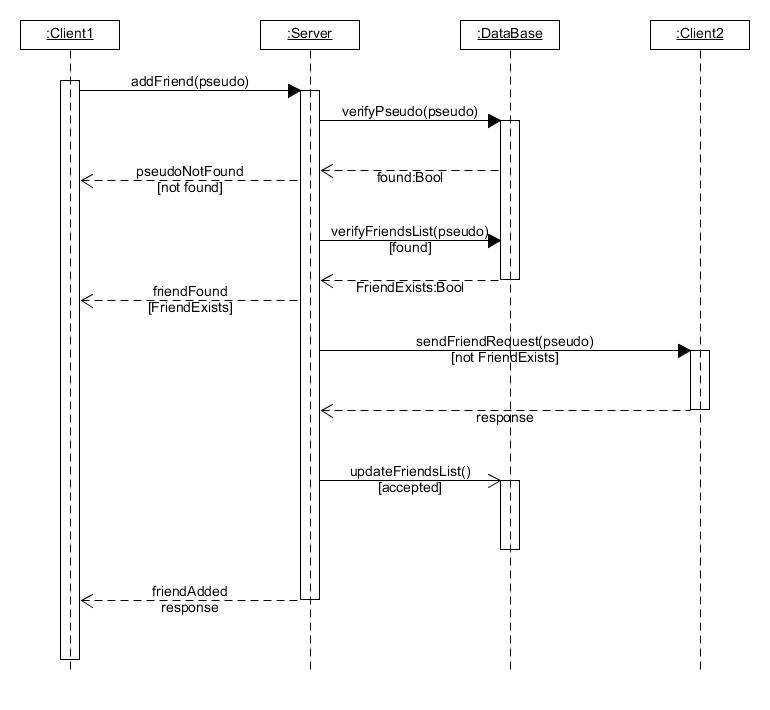
\includegraphics[scale=0.5]{images/add_friend.jpg}
\caption{Diagramme de Séquence pour l'ajout d'un ami }
\end{figure}

\begin{figure}[hbtp]
\centering
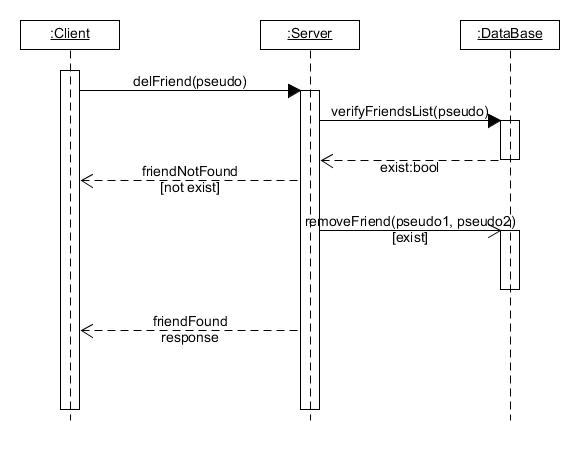
\includegraphics[scale=0.5]{images/del_friend.jpg}
\caption{Diagramme de Séquence pour la suppression d'un ami }
\end{figure}


\begin{figure}[hbtp]
\centering
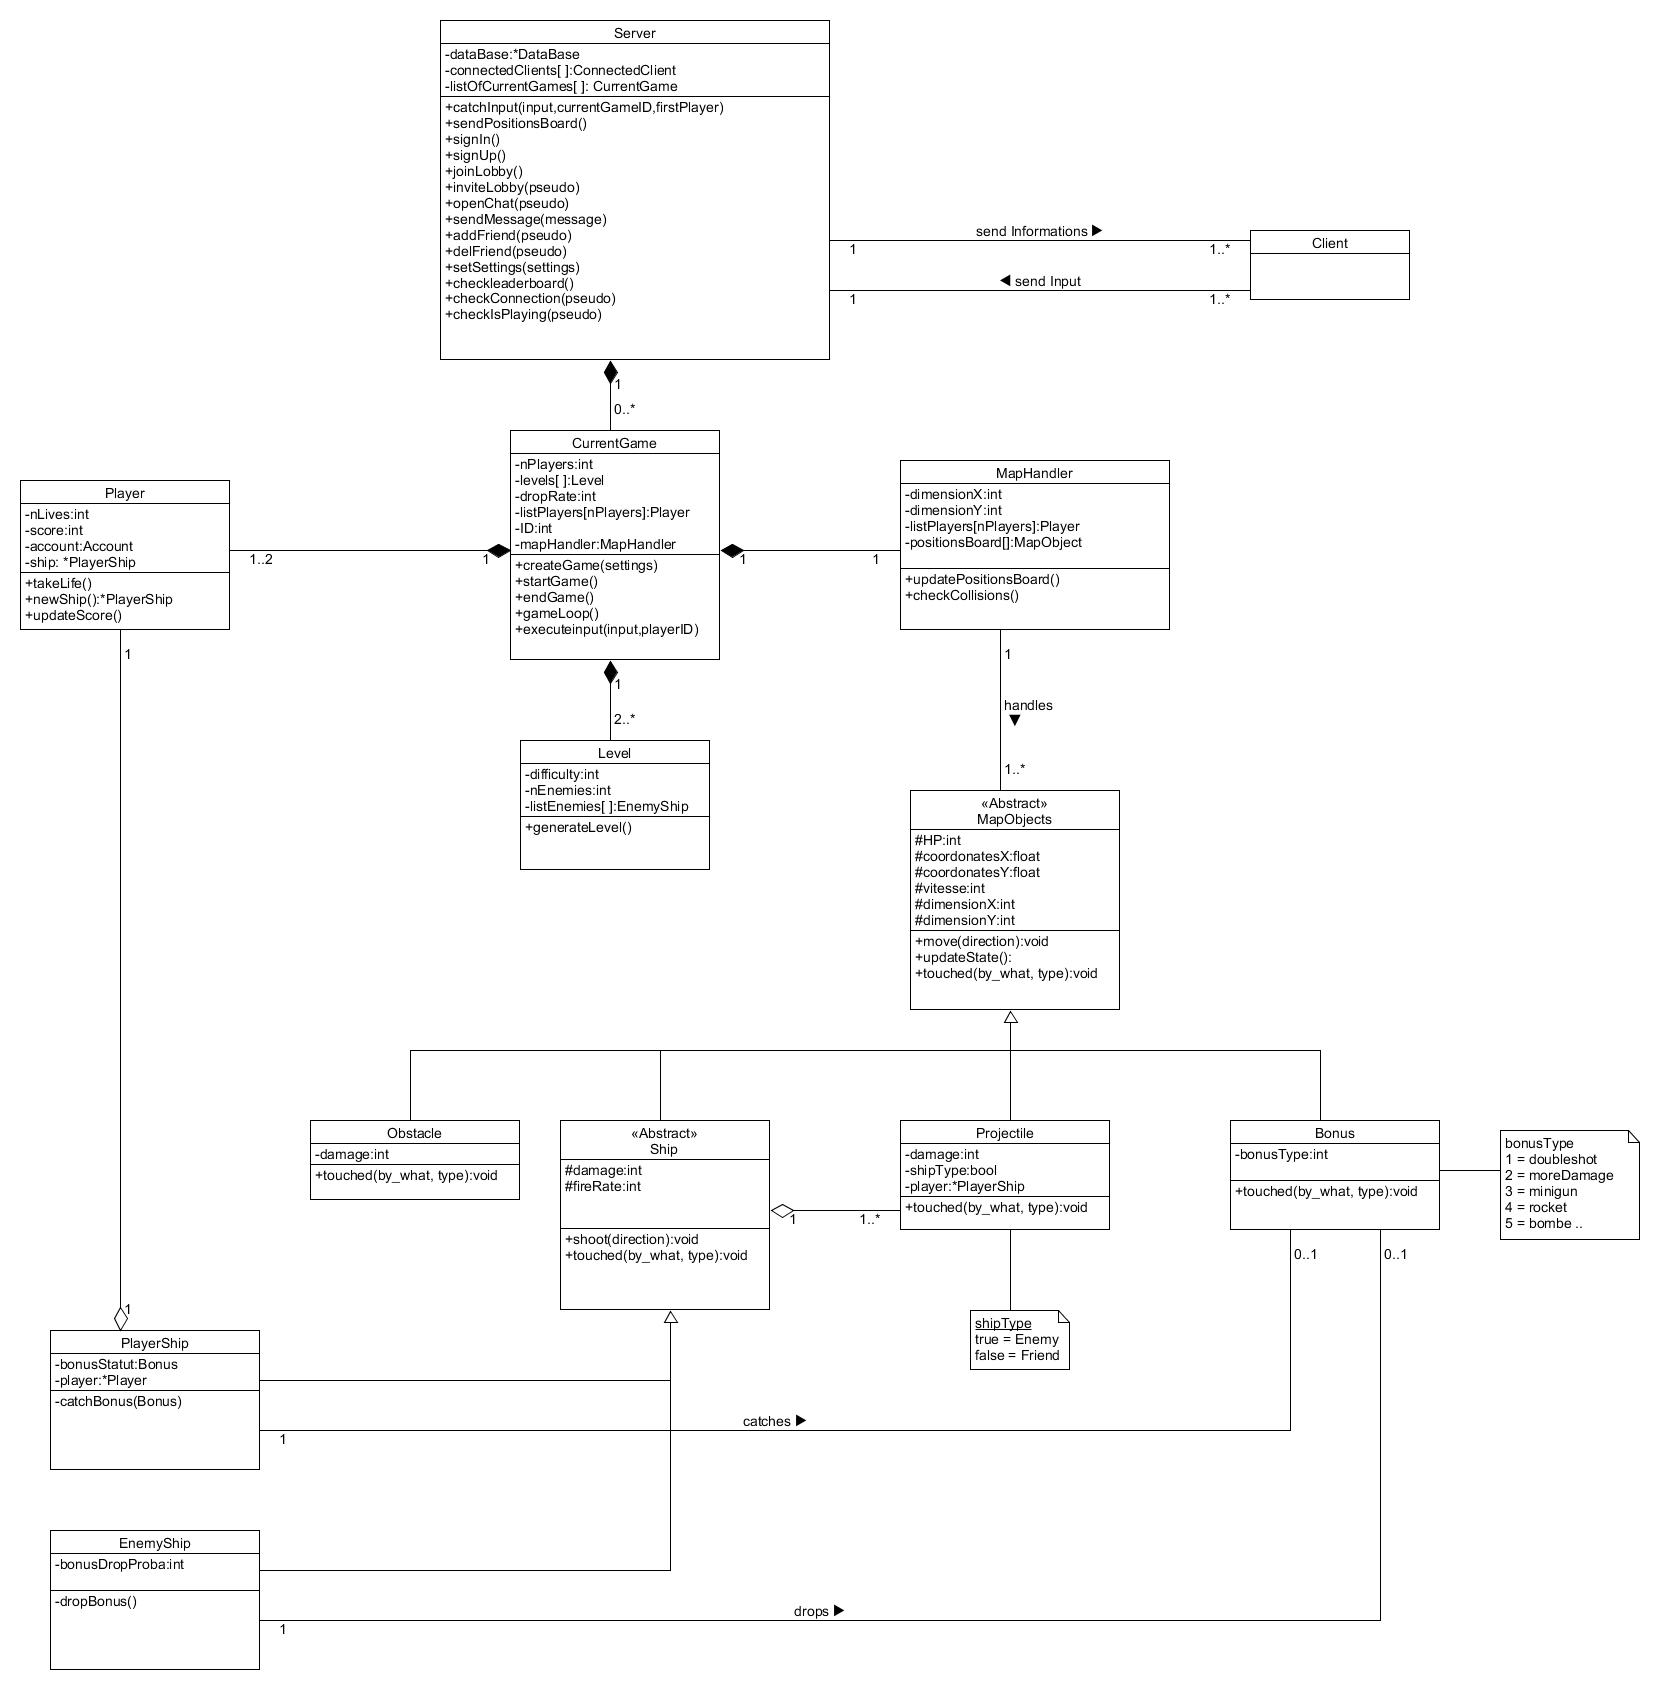
\includegraphics[scale=0.3]{images/newGameClassDiagram.jpg}
\caption{Diagramme de Classe du jeu}
\end{figure}

\begin{figure}[hbtp]
\centering
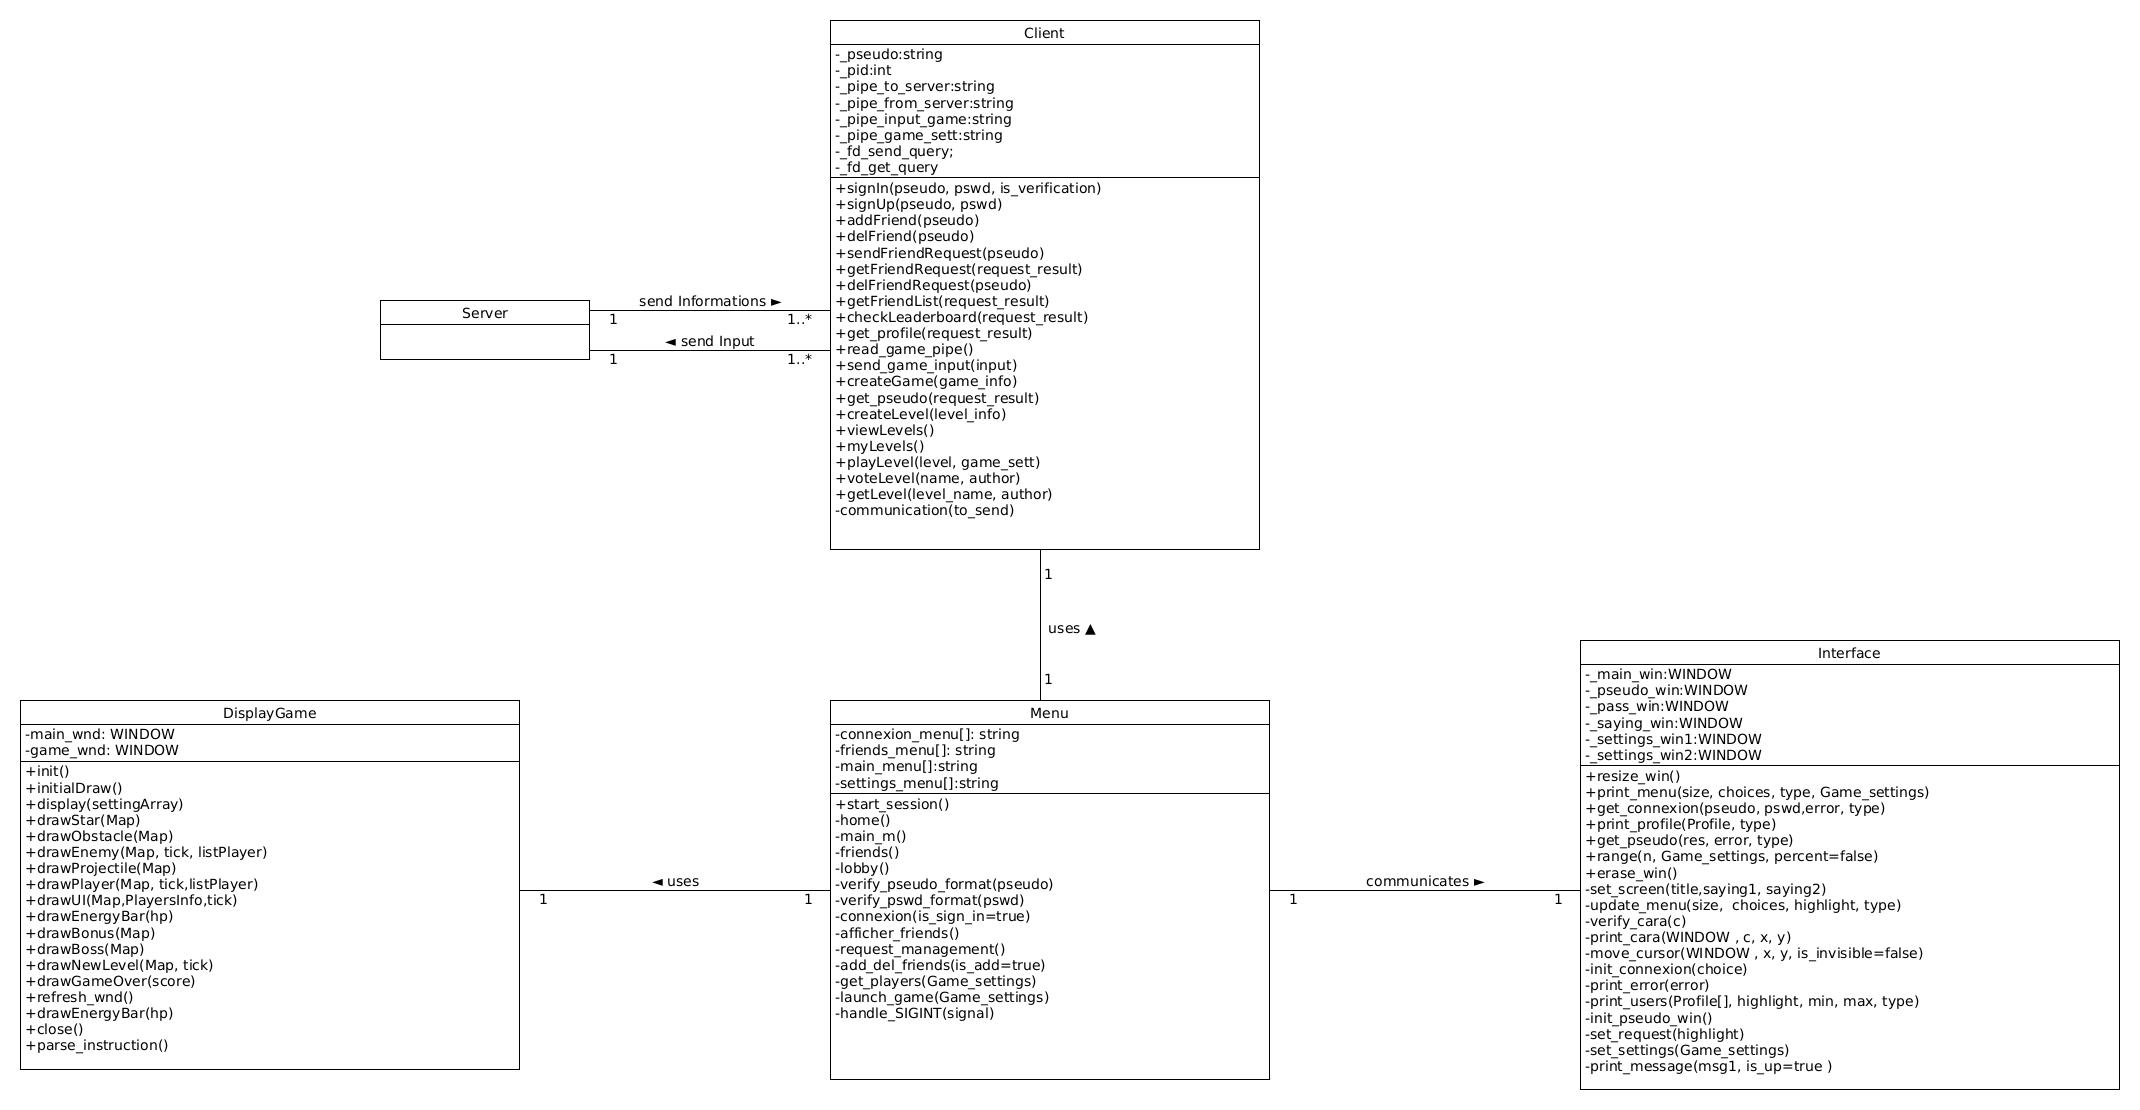
\includegraphics[scale=0.3]{images/newClientClassDiagram.jpg}
\caption{Diagramme de Classe côté Client}
\end{figure}

\newpage

\section{Besoins système}
\subsection{Besoins fonctionnels}

\begin{figure}[h!]
\centering
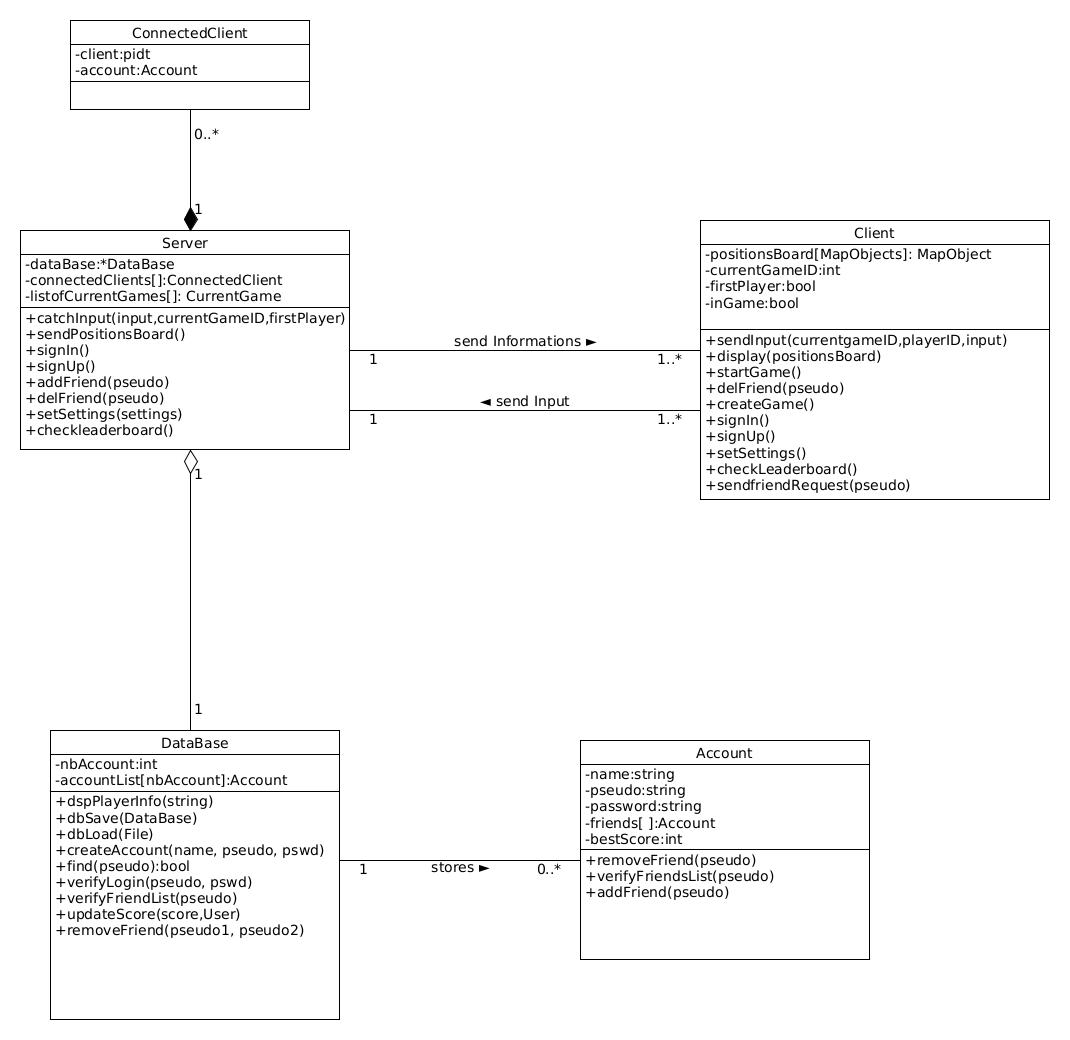
\includegraphics[width=16cm]{images/newSystemClassDiagram.jpg}
\caption{Diagramme de Classe du Système}
\label{fig:UerUseCase}
\end{figure}

\subsubsection{Serveur}
Le serveur est la classe principale du système. Il va gérer la majorité des interactions du programme et va servir d'intermédiaire entre le client et toutes les fonctionnalités du jeu. Pour le bon fonctionnement du programme, cette classe devra toujours être active.\\
Parmi les fonctionnalités principales du serveur, on peut trouver:\\
- La connexion entre client et serveur\\
- L'interaction entre les utilisateurs\\
- La gestion des données personnelles\\
- La gestion de la partie en cours 
\subsubsection{DataBase}
Cette classe sauvegardera toutes les informations persistantes et nécessaires au bon fonctionnement du jeu.\\
Elle se chargera de:\\
- préserver et manipuler les informations personnelles relatives à chaque joueur\\
- la vérification de l'existence des données

\subsubsection{Client}
La classe Client permet à l'utilisateur de communiquer avec le serveur à travers diverses actions possibles affichées grâce au menu.
Toutes les fonctionnalités décrites dans la section 2.1 sont possibles :
\begin{itemize}
    \item Se connecter
    \item S'inscrire
    \item Créer une partie
    \item Consulter le classement
    \item Ajouter ou supprimer un ami
\end{itemize}

Les actions citées ne sont possibles que si le client est connecté au serveur. Les entrées du client sont capturées par la classe Input.\\
La classe Input est connectée au menu affiché à l'écran, ce qui permet de transmettre les entrées au client qui les enverra ensuite au serveur.\\
La classe abstraite Menu a pour but de représenter une interface au niveau graphique ou terminal. Les classes héritières de la classe abstraite devront afficher le menu qui leur correspond et vérifier à la demande de la classe Input la validité d'une entrée.\\
La classe Display permet de gérer l'affichage des objets du jeu pour le client.


\subsubsection{Gestion des comptes}
Un objet Account contient toutes les informations relatives à un utilisateur (pseudo, mot de passe, etc). Ces informations sont stockées dans la base de données et les différentes demandes d'accès à celle-ci sont traitées par le serveur.

- Accès:

Lors de la création d'un compte, la disponibilité du pseudo est vérifiée par le serveur. Si celui-ci n'est pas trouvé, un nouveau compte est bien créé et ajouté dans la base de données.

Lors de la connexion, c'est encore le serveur, à travers la base de données qui vérifie que le pseudo et le mot de passe saisis correspondent à un compte existant.

- Contenu d'un compte:

Chaque compte possède des informations sur l'utilisateur auquel il appartient, notamment ses identifiants (pseudo, mot de passe), son score (pour qu'il apparaisse dans le classement général des joueurs) et une liste d'amis qu'il peut consulter à tout moment.

\subsubsection{Gestion d'une partie}

Lorsque le joueur voudra lancer une partie,
il aura la possibilité de choisir les paramètres de celle-ci comme expliqué plus haut (cf 2.1.3). Si le nombre de joueurs choisi est 2, l'hôte doit obligatoirement inviter un autre utilisateur à se connecter.

La partie ne peut pas commencer tant que le second joueur ne réussit pas à se connecter.
\subsubsection{Gestion des amis}

- Ajout: Lorsque l'utilisateur veut ajouter un ami, le serveur effectue des vérifications et envoie la demande, si elle est valide, à la personne concernée. Si la demande est acceptée, la liste d'amis des deux utilisateurs est mise à jour par le serveur.

- Suppression: Le serveur fait une recherche de l'ami à supprimer et l'efface de la liste d'amis de l'utilisateur. L'utilisateur sera également supprimé de la liste de son ancien ami.


\subsubsection{Classement}

Après chaque partie, le serveur met à jour le score de chaque joueur si celui-ci est supérieur à son score actuel.

\subsection{Besoins non fonctionnels}

- Le lancement du programme nécessite un environnement Linux.\\
- Par souci de sécurité, toutes les requêtes d'un client doivent passer par le serveur.


\begin{figure}[hbtp]
\centering
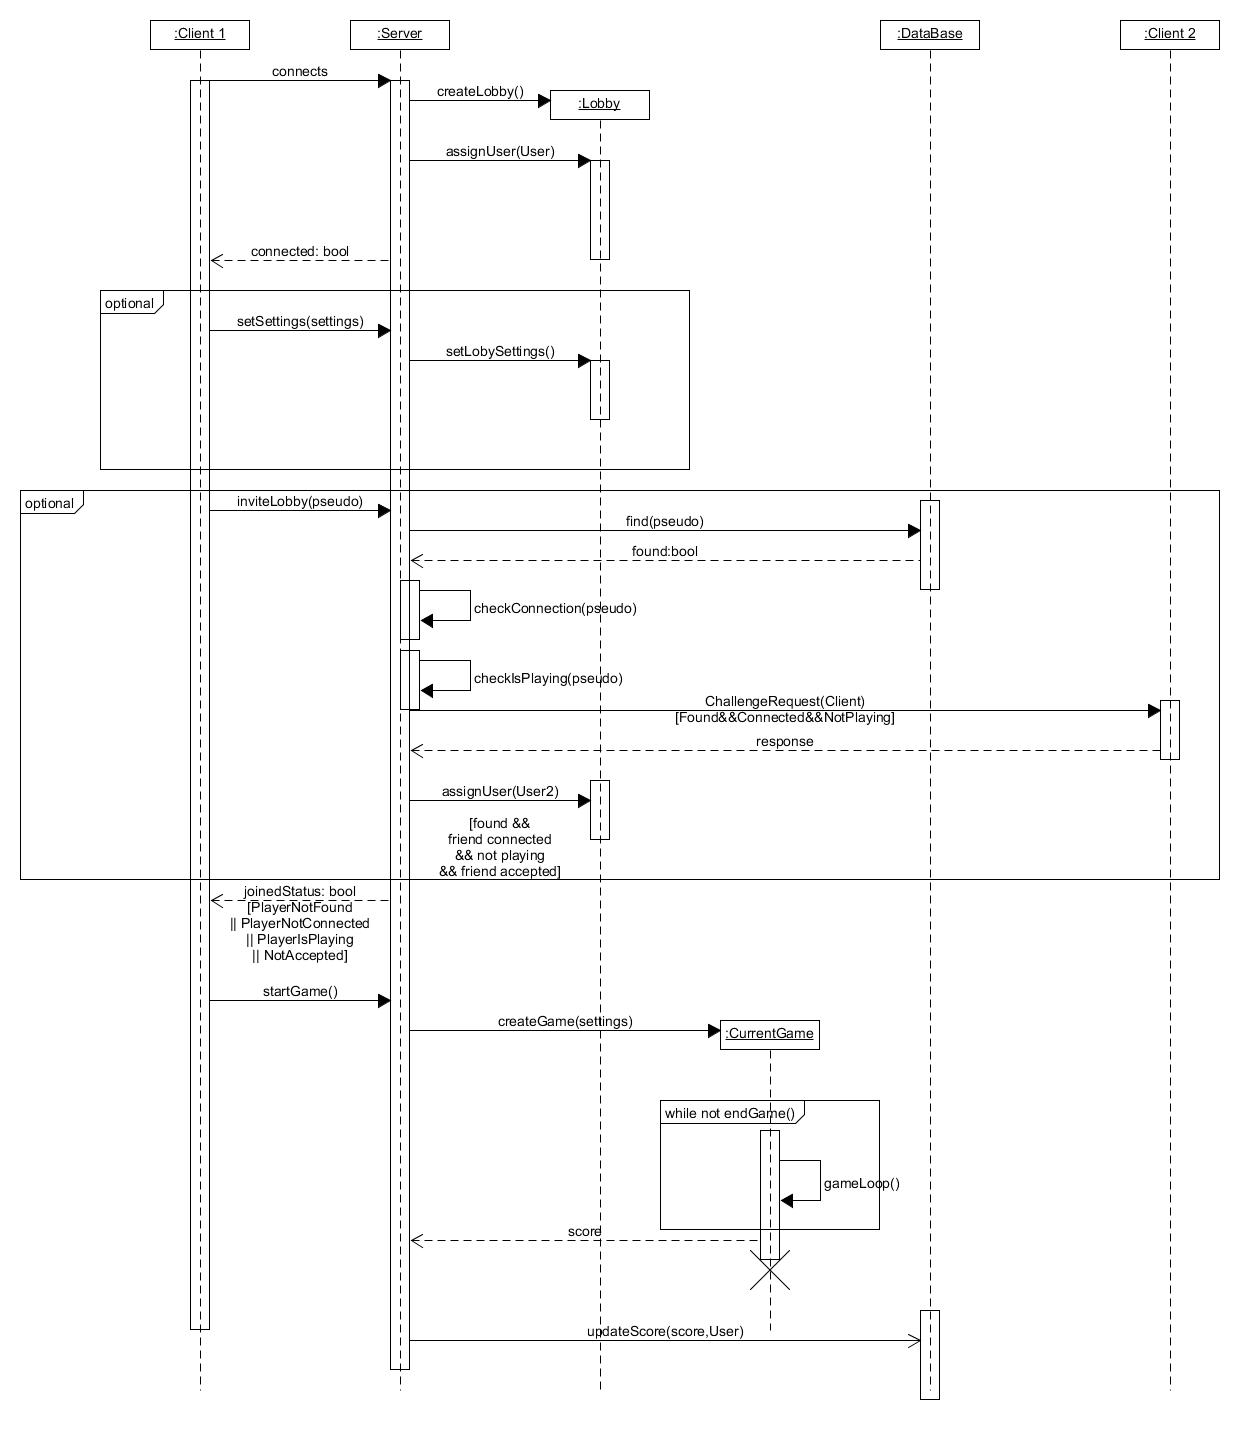
\includegraphics[scale=0.3]{images/sequence_diagram_StartGame}
\caption{Diagramme de Séquence de lancement du jeu}
\end{figure}

\begin{figure}[hbtp]
\centering
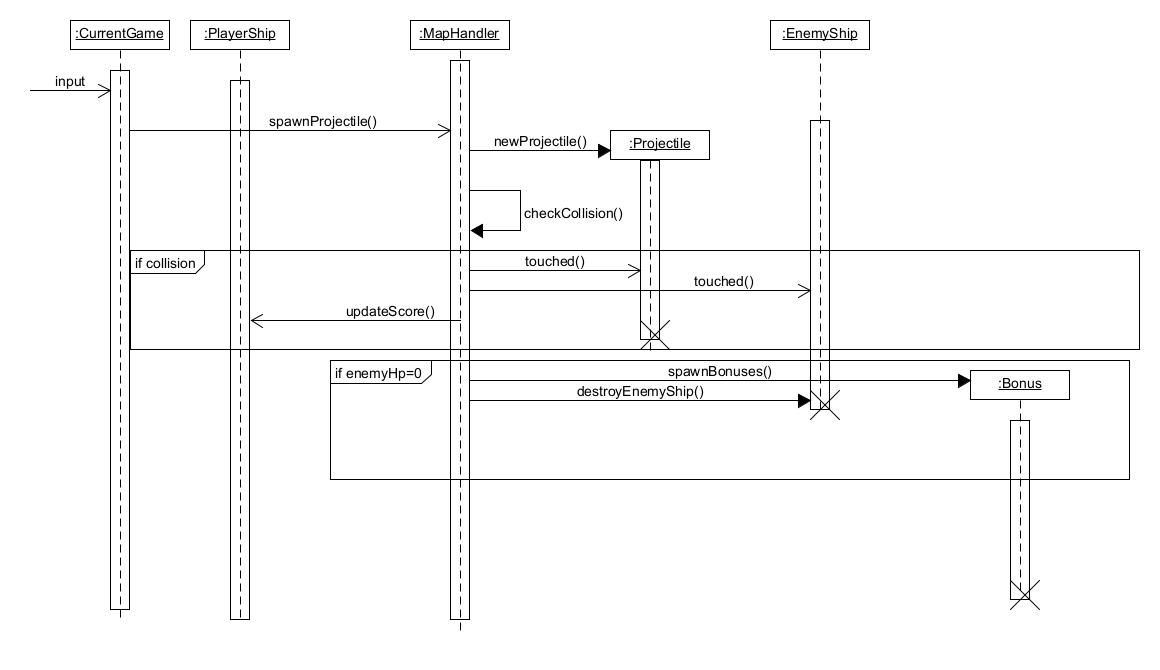
\includegraphics[scale=0.3]{images/player_shooting.jpg}
\caption{Diagramme de Séquence d'un tir de joueur}
\end{figure}


\begin{figure}[hbtp]
\centering
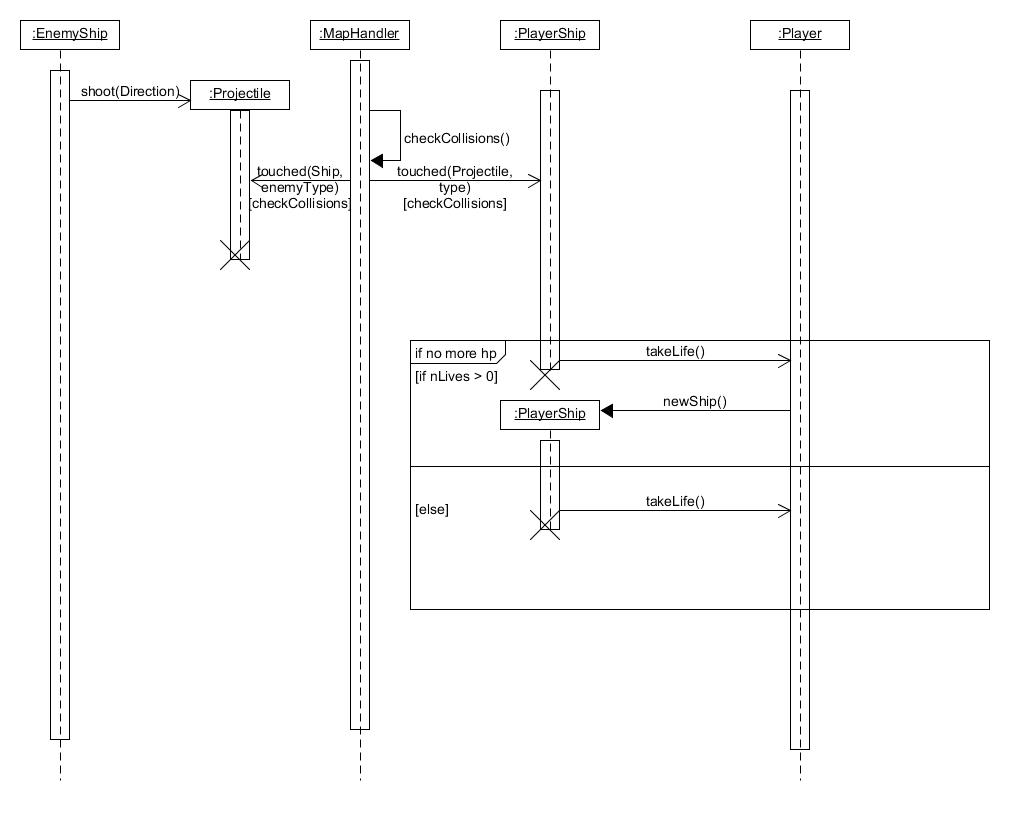
\includegraphics[scale=0.3]{images/enemy_shooting.jpg}
\caption{Diagramme de Séquence d'un tir ennemi }
\end{figure}

\newpage
\section{Annexes}
\subsection{ Description du diagramme Use Case utilisateur}

\begin{center}
\begin{longtable}{|p{1,5cm}||p{3,5cm}|p{3,5cm}|p{3,5cm}|p{3,5cm}|}
\hline
\rowcolor{green}
USE CASE   &\center{Pré-conditions}   & \hfill Post-conditions \hfill\null & Cas Général & Cas exceptionnels\\
\hline
\hline
\textbf{Sign in}      & L'utilisateur doit être enregistré dans la base de données  & L'utilisateur est connecté à sa base de données et le menu principal est affiché & L'utilisateur déjà enregistré se connecte à son compte en entrant son pseudonyme et mot de passe. Le serveur vérifie que les données soient correctes et donne accès au compte du client  & Si l’identifiant ou le mot de passe sont incorrects, affiche un message d'erreur est affiché à l'utilisateur \\
\hline
\hline
\textbf{Sign up}     & L'utilisateur n'est pas présent dans la base de données   & Ajout d'un compte dans la base de données et affichage du menu principal & L'utilisateur crée un compte en introduisant un pseudo et un mot de passe  & Si les données entrées ne respectent pas le format requis ou que le pseudonyme est déjà utilisé, un message d'erreur est affiché et l'utilisateur peut recommencer l'action jusqu'à ce qu'elle soit valide \\

\hline
\hline
\textbf{Create game}    & L'utilisateur doit être enregistré dans la base de données  & Possibilité de sauvegarder les paramètres par défaut d'une partie  & L'utilisateur peut lancer une partie après avoir rempli les conditions minimales  & Néant \\
\hline
\hline
\textbf{Check Leaderboard}  & L'utilisateur doit être enregistré dans la base de données   & \hfill Néant  \hfill\null &Le joueur peut consulter le classement des scores en envoyant une requête au serveur qui va lui renvoyer les informations  & Néant \\
\hline
\hline
\textbf{View friend list }   & L'utilisateur doit être enregistré dans la base de données   & Néant  & Consultation de liste d'ami dans la base de données & Néant \\
\hline
\hline
\textbf{Add friend}    & L'utilisateur doit être enregistré dans la base de données   & Si invitation acceptée, ajout d'amis dans la base de donnée (bidirectionnel) & Entrer le pseudo d’un utilisateur. Le système va rechercher dans la base de données si le pseudo existe et lui envoyer une invitation.  & Ajouter un pseudo qui n’existe pas (affiche une erreur)\\
\hline
\hline
\textbf{Delete friend}    & L'utilisateur doit être enregistré dans la base de données et avoir au moins un ami.   & Suppression dans la liste d’amis par le serveur(bidirectionnel)  & Entrer le pseudo d’un ami. Le serveur va rechercher dans la base de données si le pseudo existe et le supprimer.  & Supprimer un ami qui n’existe pas (affiche une erreur) \\
\hline
\hline
\textbf{Settings}     & L'utilisateur doit être enregistré dans la base de données   & Mise à jour des changements  & L'utilisateur peut modifier ses paramètres de profil et/ou audiovisuels. Il peut également consulter les règles du jeu  & Néant\\
\hline
\hline
\textbf{Ship’s controls}  & Créer une partie  & Actualisation de l’état de jeu  & Se déplacer, tirer recevoir des bonus  & Néant\\
\hline
\hline
\textbf{Leave party}      & Être en train de jouer   & Retour au menu principal  & Le joueur arrête la partie en cours.  & Néant\\
\hline
\hline
\hline
\hline
\textbf{Leave game}      & Etre connecté   & Fermeture du jeu  & L'utilisateur est connecté et veut quitter le jeu  & L'utilisateur est connecté et force sa sortie du jeu (CTRL+C, ...)\\
\hline
\end{longtable}
\end{center}


\end{document}
